\section{Localization}
\label{App:localization}
In \autoref{HallCombArrows} we propose that the maps appearing in the combinatorial Hall algebra construction should be in a kind of localization of $\lSet$. 

Here we describe this kind of structure more generally, and not very rigorously.

Let $\DDD$ be a category, and $W$ some class of "weak equivalences". As usual we denote maps in $W$ by $\xrightarrow{\sim}$. We construct a double category $\DDD_W$ as follows:
\begin{itemize}
    \item Objects are objects of $\DDD$.
    \item Morphisms $A$ to $B$ are diagrams of the form $A\xleftarrow{\sim}E\to B$.
    \item Squares are commutative diagrams of the form
    \[
   \stik{1}{
    A \& E \ar{l}[above,sloped]{\sim} \ar{r}{} \& B \\
    F \ar{u}[above,sloped]{\sim} \ar{d}{}\& Z \ar[leftarrow]{ul} \ar[leftarrow]{ur} \ar[leftarrow]{dl} \ar[leftarrow]{dr}[above,sloped]{\sim}\& G\ar{u}[above,sloped]{\sim} \ar{d} \\
    C \& H \ar{l}[above,sloped]{\sim} \ar{r} \& D \\
    }
    \]
\end{itemize}

\begin{Remark}
If a functor $\DDD\xrightarrow{\phi}\CCC$ maps $W$ to isomorphisms, then it factors through $\DDD_W$ with the functor $\DDD_W\xrightarrow{\phi_W}\CCC$ being defined by
\[
A\xleftarrow{\stackrel{\alpha}{\sim}}E\xrightarrow{f} B\mapsto \phi(A)\xrightarrow{\phi(f)\phi(\alpha)^{-1}}\phi(B)
\]
It is then easy to check that squares go to commutative squares.
\end{Remark}

\subsection{Some conditions on \texorpdfstring{$W$}{W}}
For $\DDD_W$ as described to be closed on composition of morphisms and squares we can require the following of $W$:
\begin{itemize}
    \item $W$ is stable under pullback and pushout by any morphism in $\DDD$.
    \item All morphisms in $W$ are epimorphisms in $\DDD$.
\end{itemize}

\subsection{Transfer}

If we have a transfer theory from $\DDD$ then it can be extended to a transfer from $\DDD_W$ in a straightforward way.

\subsection{Correspondences}

It is straightforward to extend the construction of $\Corr(\DDD)$ to get a double category $\Corr(\DDD_W)$ where we replace the commutative squares by squares in $\DDD_W$. 
This is the form of what we get in \autoref{HCombSquares}.

\subsection{Weak equivalences in \texorpdfstring{$\lSet$}{lSet}}

Currently we don't have a good description of what we would like to call weak equivalences in general in $\lSet$, but we have many examples, such as the one we saw above:

\[
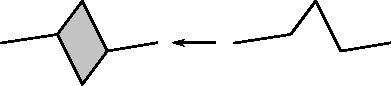
\includegraphics{Figures/lSetEquivs.pdf}
\]

Most likely it would be helpful if this is part of a model structure on $\lSet$.
